\chapter{Interface para Protocolos de Aplicação}
\label{chapter:interface_iot}

No capítulo \ref{chapter:intro}, foram vistos as bases para se implementar um projeto de IoT. A área começou a receber fortes investimentos e atenção por volta de 2009 e desde então foram feitas consideráveis implementações utilizando tecnologias e protocolos diferentes. Neste capítulo serão apresentados algumas dessas variantes, para fins de comparação e respaldo para importância e objetivo deste projeto.

Inicialmente, os conceitos e ideias do projeto eram voltados a desenvolver uma interface no qual um desenvolvedor poderia implementar um sistema IoT de ponta a ponta utilizando APIs que direcionariam para um desses protocolos da seção \ref{section:tecnologias_iot}, porém as diferenças entre os protocolos e as camadas de base, fazem com que esta solução esteja mais distante. Então o foco voltou-se  para tecnologias que tenham base na pilha TCP/IP, por sua vasta implementação nas redes industriais e residências e na Internet.

Neste projeto será visto a implementação desta interface para o protocolo MQTT, entretanto a idéia é estender o interfaceamento com outros protocolos com caracterísitcas favoráveis para uma rede IoT, como mostrado na \ref{fig:2.2.0/camada_abatracao}, assim como apresentar uma estrutura que se traduza aos protocolos sobre o TCP/IP. Algumas características fundamentais podem ser destacadas como fundamentais:

\begin{itemize}

\item Full-Duplex. Capaz de receber e enviar mensagens ao mesmo tempo;
\item Multicast. Capaz de enviar mensagens um ou mais dispositivos simultâneos;
\item Envio de mensagens em tempo real;

\end{itemize}


\begin{figure}[h!]
\centering
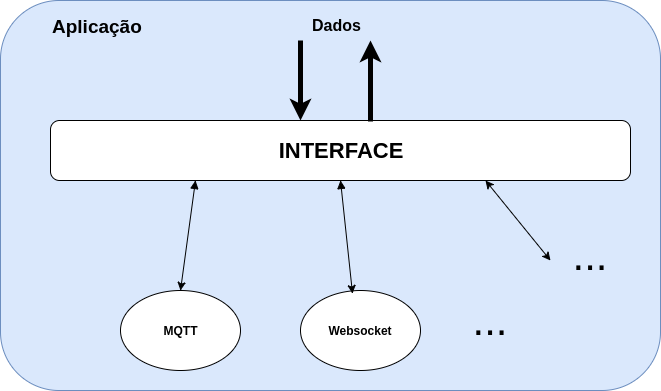
\includegraphics[width=12cm]{./02_Capitulos/02_Cap2/figures/camada_abstracao}
\caption{Interface de comunicação. A interface tem seu próprio protocolo que direciona e se comunica a um ou mais protocolos de aplicação}
\label{fig:2.2.0/camada_abatracao}
\end{figure}

\section{Tecnologias em IoT}
\label{section:tecnologias_iot}

As primeiras aplicações de IoT foram em laboratórios com RFID \cite{Rampim:iot}, junto com códigos bidimensionais (como o QR Code), para aplicações de identificação de objetos, é uma das soluções mais populares e de baixo custo de IoT utilizando Rádio frequência.

Redes que utilizam bandas restritas visando baixo consumo e distância de transmissão, são utiizadas em redes IoT de celulares e irão se tornar opções dominantes de conectivdade com o advento do 5G. As NB-IoT concentram-se especificamente na cobertura interna, baixo custo, longa duração da bateria e alta densidade de conexão. As mensagens de IoT são geralmente curtas, dados telemétricos, status etc. Já se encontram implementadas algumas redes como SigFox \cite{Sigfox} e LoRa \cite{LoRa}. 

As novas gerações de Bluetooth consomem muito menos energia, o que tornaram a tecnologia viável para aplicações IoT. Geralmente, módulos Bluetooth são utilizados como beacons \cite{Endeavor:Beacons}. Pontos espalhados por uma região, no qual podem se comunicar com os módulos de dispositivos mobile ao se aproximar, oferecendo links para conteúdo e exclusividades.

As tecnologias mais comuns de se encontrar em aplicações IoT, os protocolos construídos com base no TCP/IP são vastamente utilizados e possuem uma rede mundialmente distribuída, o que facilita o uso. Pode-se implementar uma gama de protocolos de aplicações, alguns mais eficientes que outros.

O protocolo mais simples seria o HTTP, altamente usado na internet, porém não é eficiente no consumo de energia por abrir uma conexão a cada envio de dados. Para minimizar estas desvantagens, foi desenvolvido o CoAP (Constrained Application Protocol) \cite{coap} protocolo nos mesmos moldes do HTTP com arquitetura REST (Representational State Transfer), que define as regras para criação de uma serviços Web, garantindo interoperabilidade entre sistemas e a Internet. Entretanto o CoAP é mais simples, mais leve, com baixo overhead e utilizado em redes locais.

Mas os mais utilizados em aplicações são sem dúvidas os protocolos que mantém conexão aberta, em especial Websocket e MQTT, sendo o primeiro mais utilizado para chats e mensagens, enquanto o segundo domina o mundo do M2M e Telemetria.







